\begin{frame}[fragile]
\frametitle{LA-CoNGA es}
\begin{columns}[c] % The "c" option specifies centered vertical alignment while the "t" option is used for top vertical alignment

\column{.54\textwidth}
\begin{itemize}
\item LA-CoNGA-physics: {\bf L}atin {\bf A}merican alliance for {\bf C}apacity buildi{\bf NG} in {\bf A}dvanced physics.
\item LA-CoNGA physics {\bf \color{LCredInst} es un proyecto de Capacity Building} financiado por {\bf \color{LCblueInst} Erasmus+ Programme Capacity-Building projects in the field of Higher Education (E+CBHE)}.
\item Duración: \st{3} 4 años.
\item Fecha de inicio: Enero 2020
\end{itemize}


\column{.42\textwidth} % Right column and width
\begin{center}
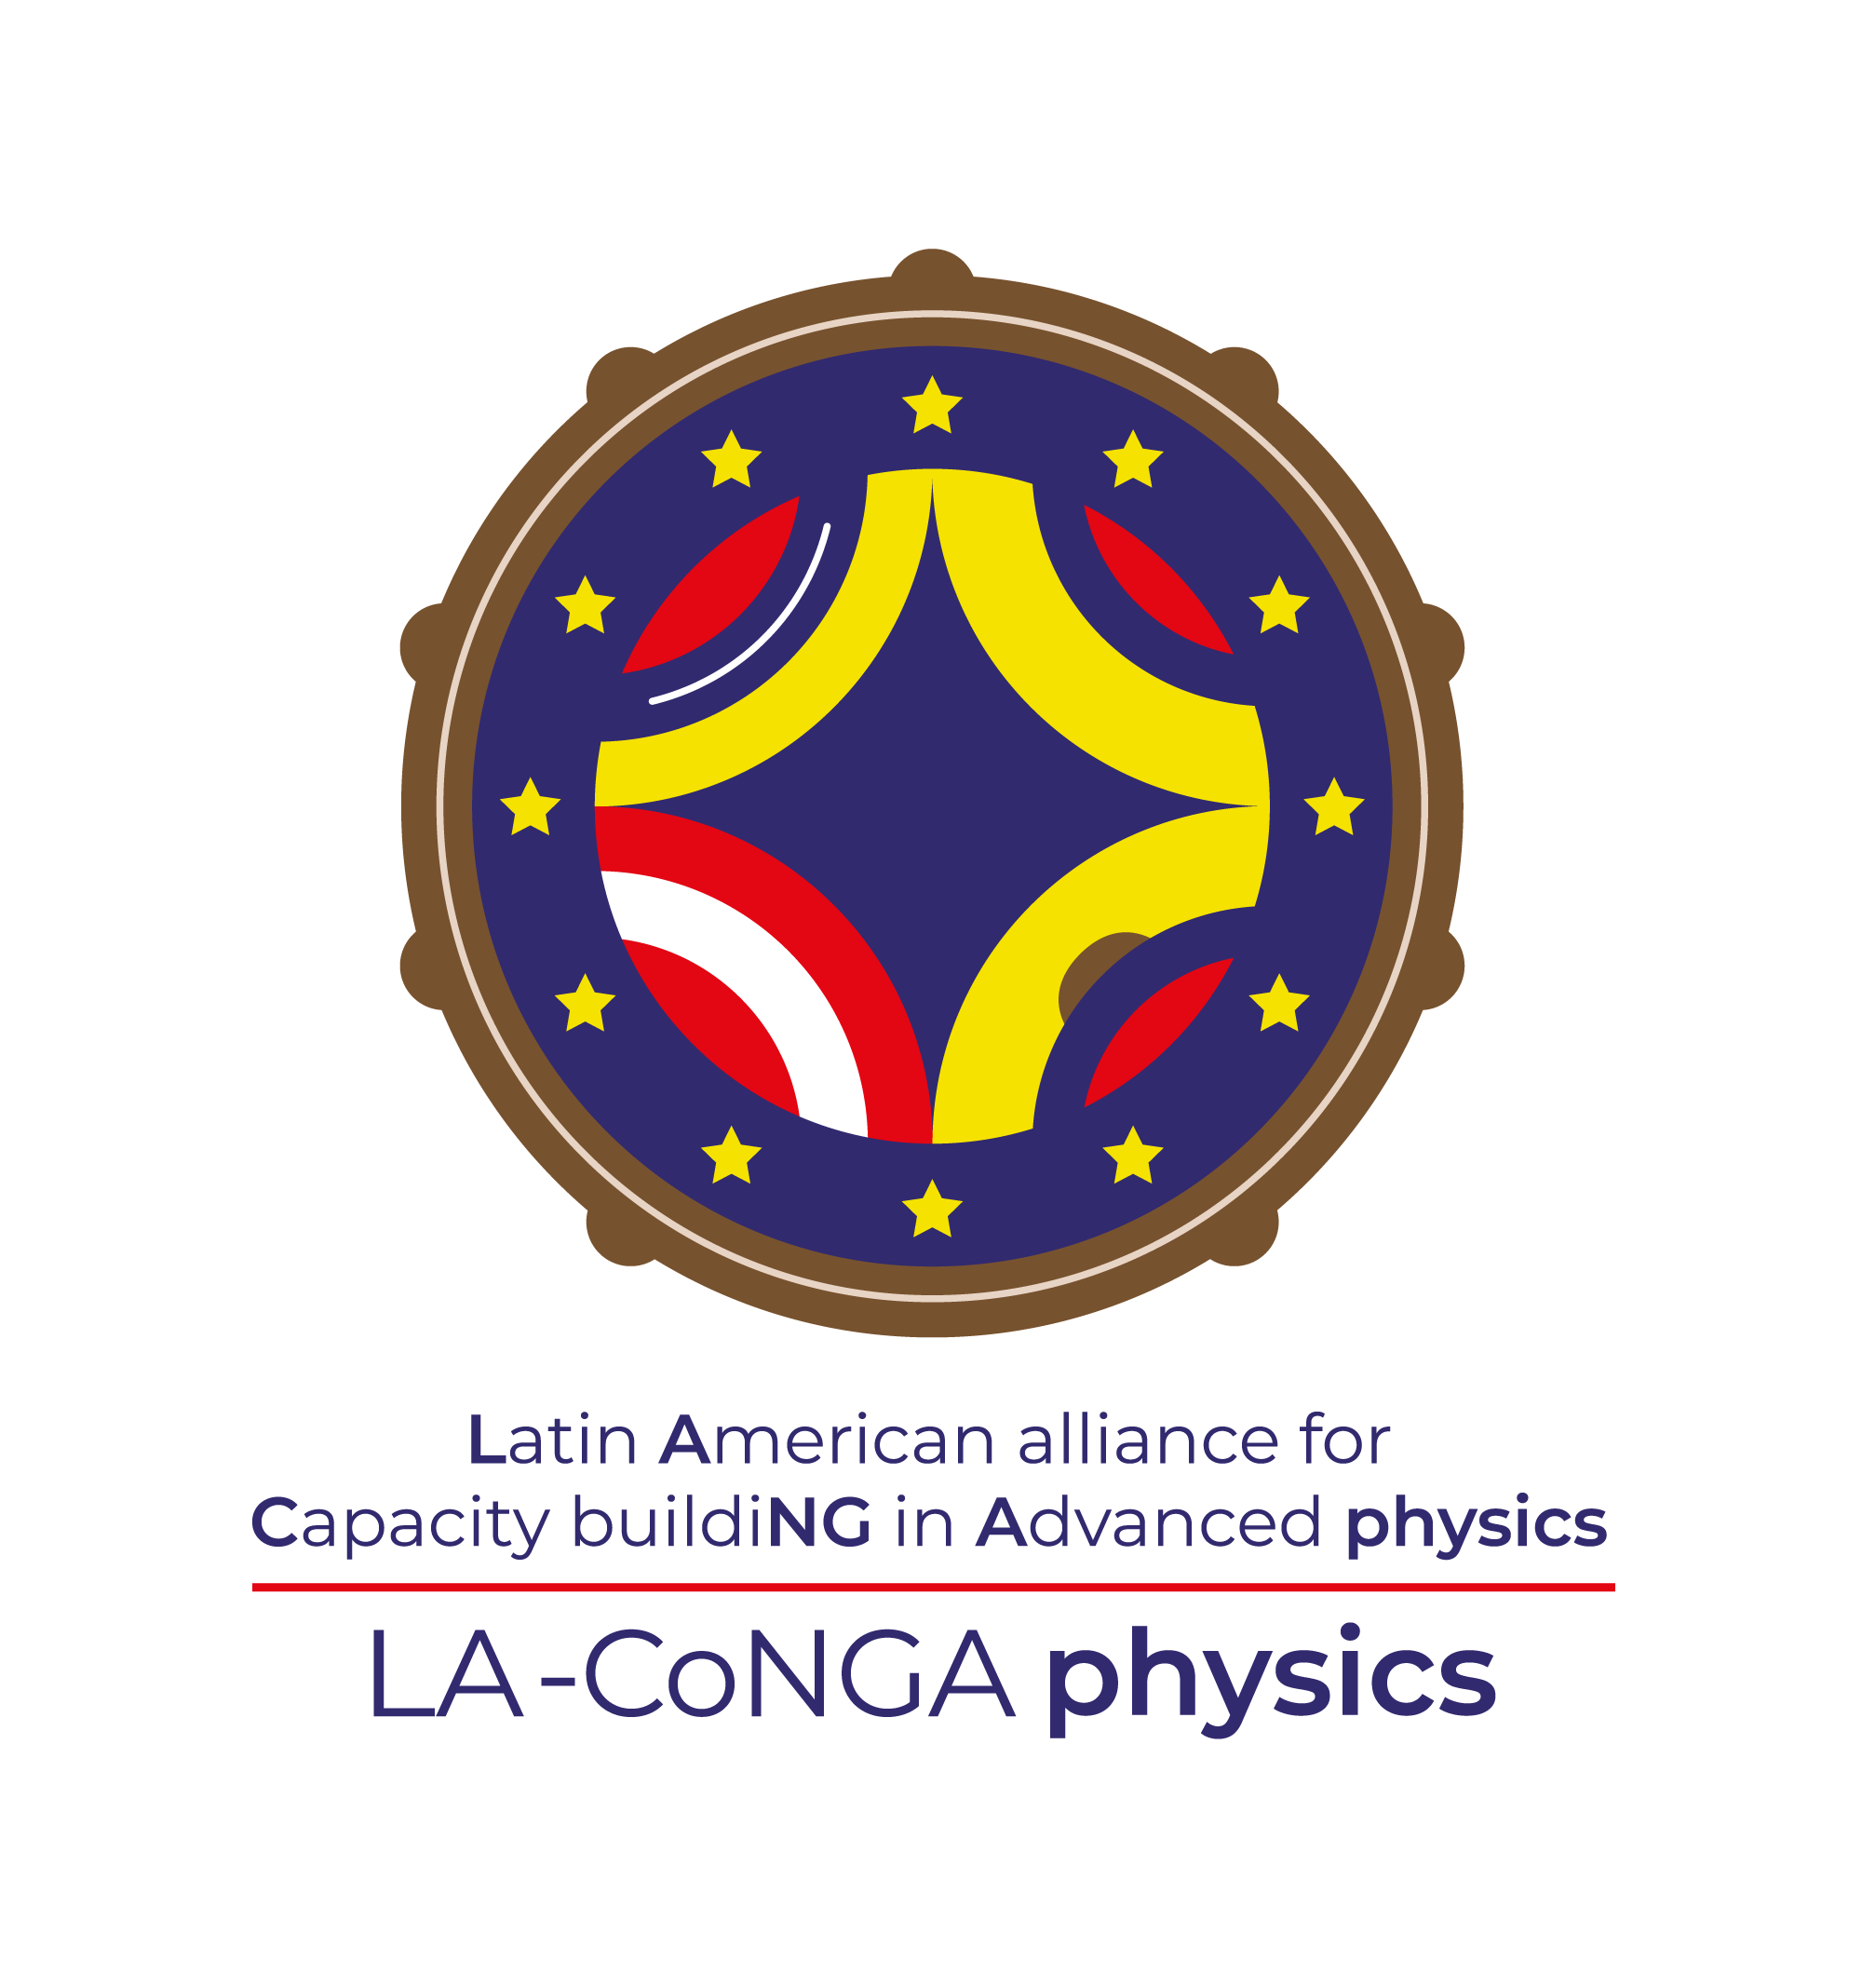
\includegraphics[scale=0.07]{imagenes/imagotipo-vertical-RGB-grande.png}
\end{center}

\end{columns}
\end{frame}

\begin{frame}<0>[fragile,noframenumbering]
\frametitle{Contexto: Sociedad del conocimiento}
\begin{columns}[c] % The "c" option specifies centered vertical alignment while the "t" option is used for top vertical alignment

\column{.38\textwidth}
En la transición a la {\bf \color{logobrown}sociedad del conocimiento} hemos encontrado: 
\begin{itemize}
\item De la sociedad {\bf \color{logoyellow}industrial} a la informacional
\item Economía {\bf \color{LCblueInst}centrada} en conocimiento
\item El conocimiento {\bf \color{LCredInst}es insumo y producto}
\item Producción {\bf \color{LCblueSec1}temprana} de conocimiento
\item Economía {\bf \color{logobrownD}global} interrelacionada
\end{itemize}


\column{.58\textwidth} % Right column and width
\begin{center}

\includegraphics[scale=0.28]{imagenes/socIndustrial.png}
\end{center}

\begin{center}
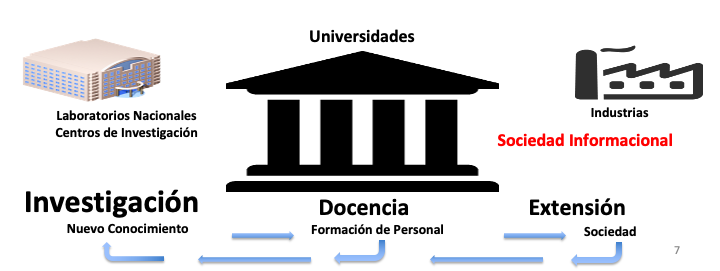
\includegraphics[scale=0.28]{imagenes/socConocimiento.png}
\end{center}
\end{columns}

\end{frame}

\begin{frame}<0>[fragile,noframenumbering]
\frametitle{Contexto: la producción del conocimiento}
\begin{columns}[c] % The "c" option specifies centered vertical alignment while the "t" option is used for top vertical alignment

\column{.38\textwidth}
La producción de conocimiento se caracteriza por ser: 
\begin{itemize}
\item Colaborativa
\item Transdisciplinar
\item Global
\item De libre acceso
\item Centrada en grandes volúmenes de datos
\end{itemize}


\column{.58\textwidth} % Right column and width
\begin{center}
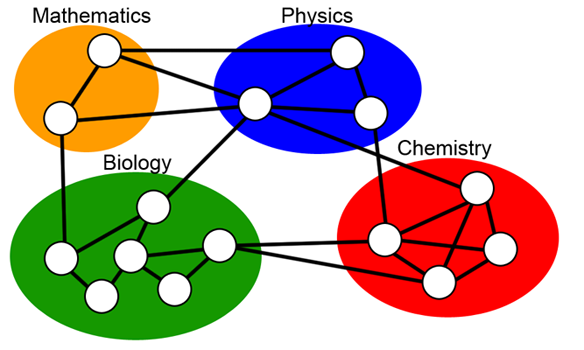
\includegraphics[scale=0.18]{imagenes/Network-of-Scientists3.png}
\end{center}

\begin{center}
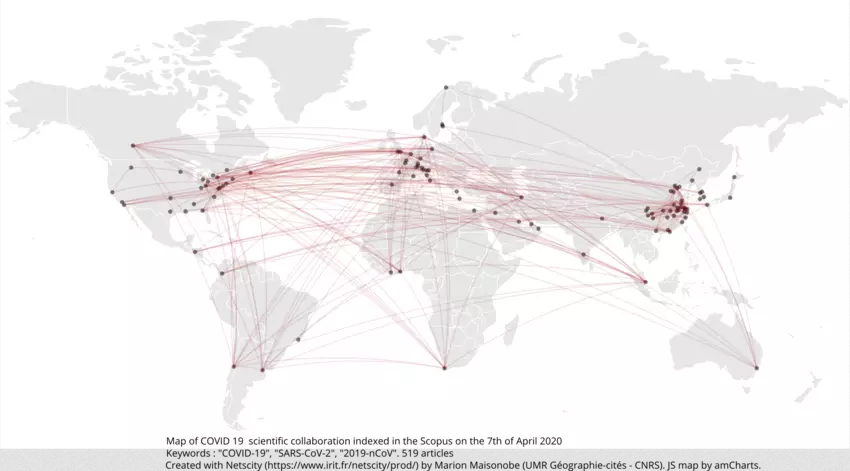
\includegraphics[scale=0.18]{imagenes/covid19_collab.png}
\end{center}
\end{columns}
\vspace{0.25cm}

{\tiny \href{https://blogs.cornell.edu/info2040/2011/09/26/scientific-collaboration-throughout-history-knowledge-networks-with-weak-local-bridges/}{\color{cyan} https://blogs.cornell.edu/info2040/2011/09/26/scientific-collaboration-throughout-history-knowledge-networks-with-weak-local-bridges/}}

{\tiny \href{https://www.weforum.org/agenda/2020/05/global-science-collaboration-open-source-covid-19/}{\color{cyan} https://www.weforum.org/agenda/2020/05/global-science-collaboration-open-source-covid-19/}}

\end{frame}

\note{Everything you want}

\begin{frame}[fragile]
\frametitle{Colaboración científica y educación a escala global}
 
\begin{itemize}
\item En la era de la información, la {\bf \color{LCblueInst}ciencia y la educación} superior se han convertido muy rápidamente en actividades {\bf \color{LCredInst}colaborativas, multidisciplinarias y distribuidas globalmente}.

\item El vínculo universidades-investigación-sociedad es más fuerte: generación de conocimiento, su aplicación y transferencia ocurren en el mismo contexto físico y social. 

\item Las {\bf \color{logoyellow}redes virtuales de investigación y aprendizaje} (Virtual Research and Learning Networks, {\bf \color{logobrownD}VRLN}) juegan un rol fundamental.

\vspace{0.5cm}

{\bf VRLN:} {\bf \color{logobrownD}Infraestructuras de información y comunicación} que combinan {\bf \color{LCredInst}datos}, herramientas de {\bf \color{LCblueInst}software y centros de investigación} para desarrollar plenamente las actividades de docencia e investigación.
\end{itemize}

\end{frame}

\begin{frame}[fragile]
\frametitle{Objetivos de una VRLN}
\begin{columns}[c] % The "c" option specifies centered vertical alignment while the "t" option is used for top vertical alignment

\column{.58\textwidth}
\begin{itemize}
\item {\bf Accesibilidad:}
Cada institución en una VRLN accede a una {\bf \color{LCredInst}cantidad mayor de recursos} y staff académico.

\item {\bf Modernización:}
Mediante el uso de las TICs y los recursos de educación abierta, conectividad, {\bf \color{LCredInst}adquisición de competencias digitales}, el uso y el desarrollo de nuevos medios de aprendizaje. Todo esto {\bf \color{LCblueInst}basado en las capacidades locales}, logrando apropiación y sostenibilidad de los proyectos.

\item {\bf Internacionalización:}
Entrenamiento de nuevas generaciones dentro de un {\bf \color{logoyellow}ambiente colaborativo internacional}.
Aumentando la diversidad en el área.

\end{itemize}


\column{.38\textwidth} % Right column and width
\begin{center}

\includegraphics[scale=0.18]{imagenes/vrln.png}
\end{center}
\end{columns}
\end{frame}

\iffalse
\begin{frame}[fragile]
\frametitle{Física de Altas Energías, Astropartículas y Cosmología en América Latina}
\begin{columns}[c] % The "c" option specifies centered vertical alignment while the "t" option is used for top vertical alignment

\column{.58\textwidth}
Me gustaría transformar esta lámina para hablar de las fortalezas regionales de ambas filiales y salir del contexto LASF4RI
\begin{itemize}
	\item High energy, cosmology and astroparticle physics (HECAP) community/activities has
undoubtedly grown in Latin America in the last decades
	\item A series of initiatives have contributed to it (non exhaustive list)
	\begin{itemize}
		\item The Pierre Auger observatory in Argentina
		\item HELEN and EPLANET programs
		\item Several other national, bi-national or multinational projects
		\end{itemize}
	\item In terms of human and research resources the HECAP development is nuanced and
variable country-by-country (this impacts the training of the new generations)
	\begin{itemize}
		\item Diversity of interests and skills developed (as we see in this forum!)
		\item A young generation with much potential and eagerness to learn
		\item Together we are stronger
		\end{itemize}
	\item HEP is one of the thematic areas of LA-CoNGA physics (another one is complex systems)
\end{itemize}


\column{.38\textwidth} % Right column and width
\begin{center}

\includegraphics[scale=0.18]{imagenes/vrln.png}
\end{center}
\end{columns}
\end{frame}
\fi

\begin{frame}[fragile]
\frametitle{\underline{Misión}, Visión y Valores}
\begin{columns}[c] % The "c" option specifies centered vertical alignment while the "t" option is used for top vertical alignment

\column{.56\textwidth}
Nuestra {\bf\Large \color{LCredInst} misión} es {\bf \color{LCblueSec1} crear una \underline{Comunidad} Latinoamericana y Europea \underline{de Investigación y Aprendizaje} de Física Avanzada} para desarrollar capacidades, {\bf \color{logoyellow} \underline{apoyando la modernización} del sistema de educación superior} y promoviendo valores de {\bf \color{logobrown} colaboración, educación e investigación abierta en \underline{universidades} y \underline{organismos} de \underline{investigación} de \underline{Colombia}, \underline{Ecuador}, \underline{Perú} y \underline{Venezuela}}.

\column{.40\textwidth} % Right column and width

\begin{center}
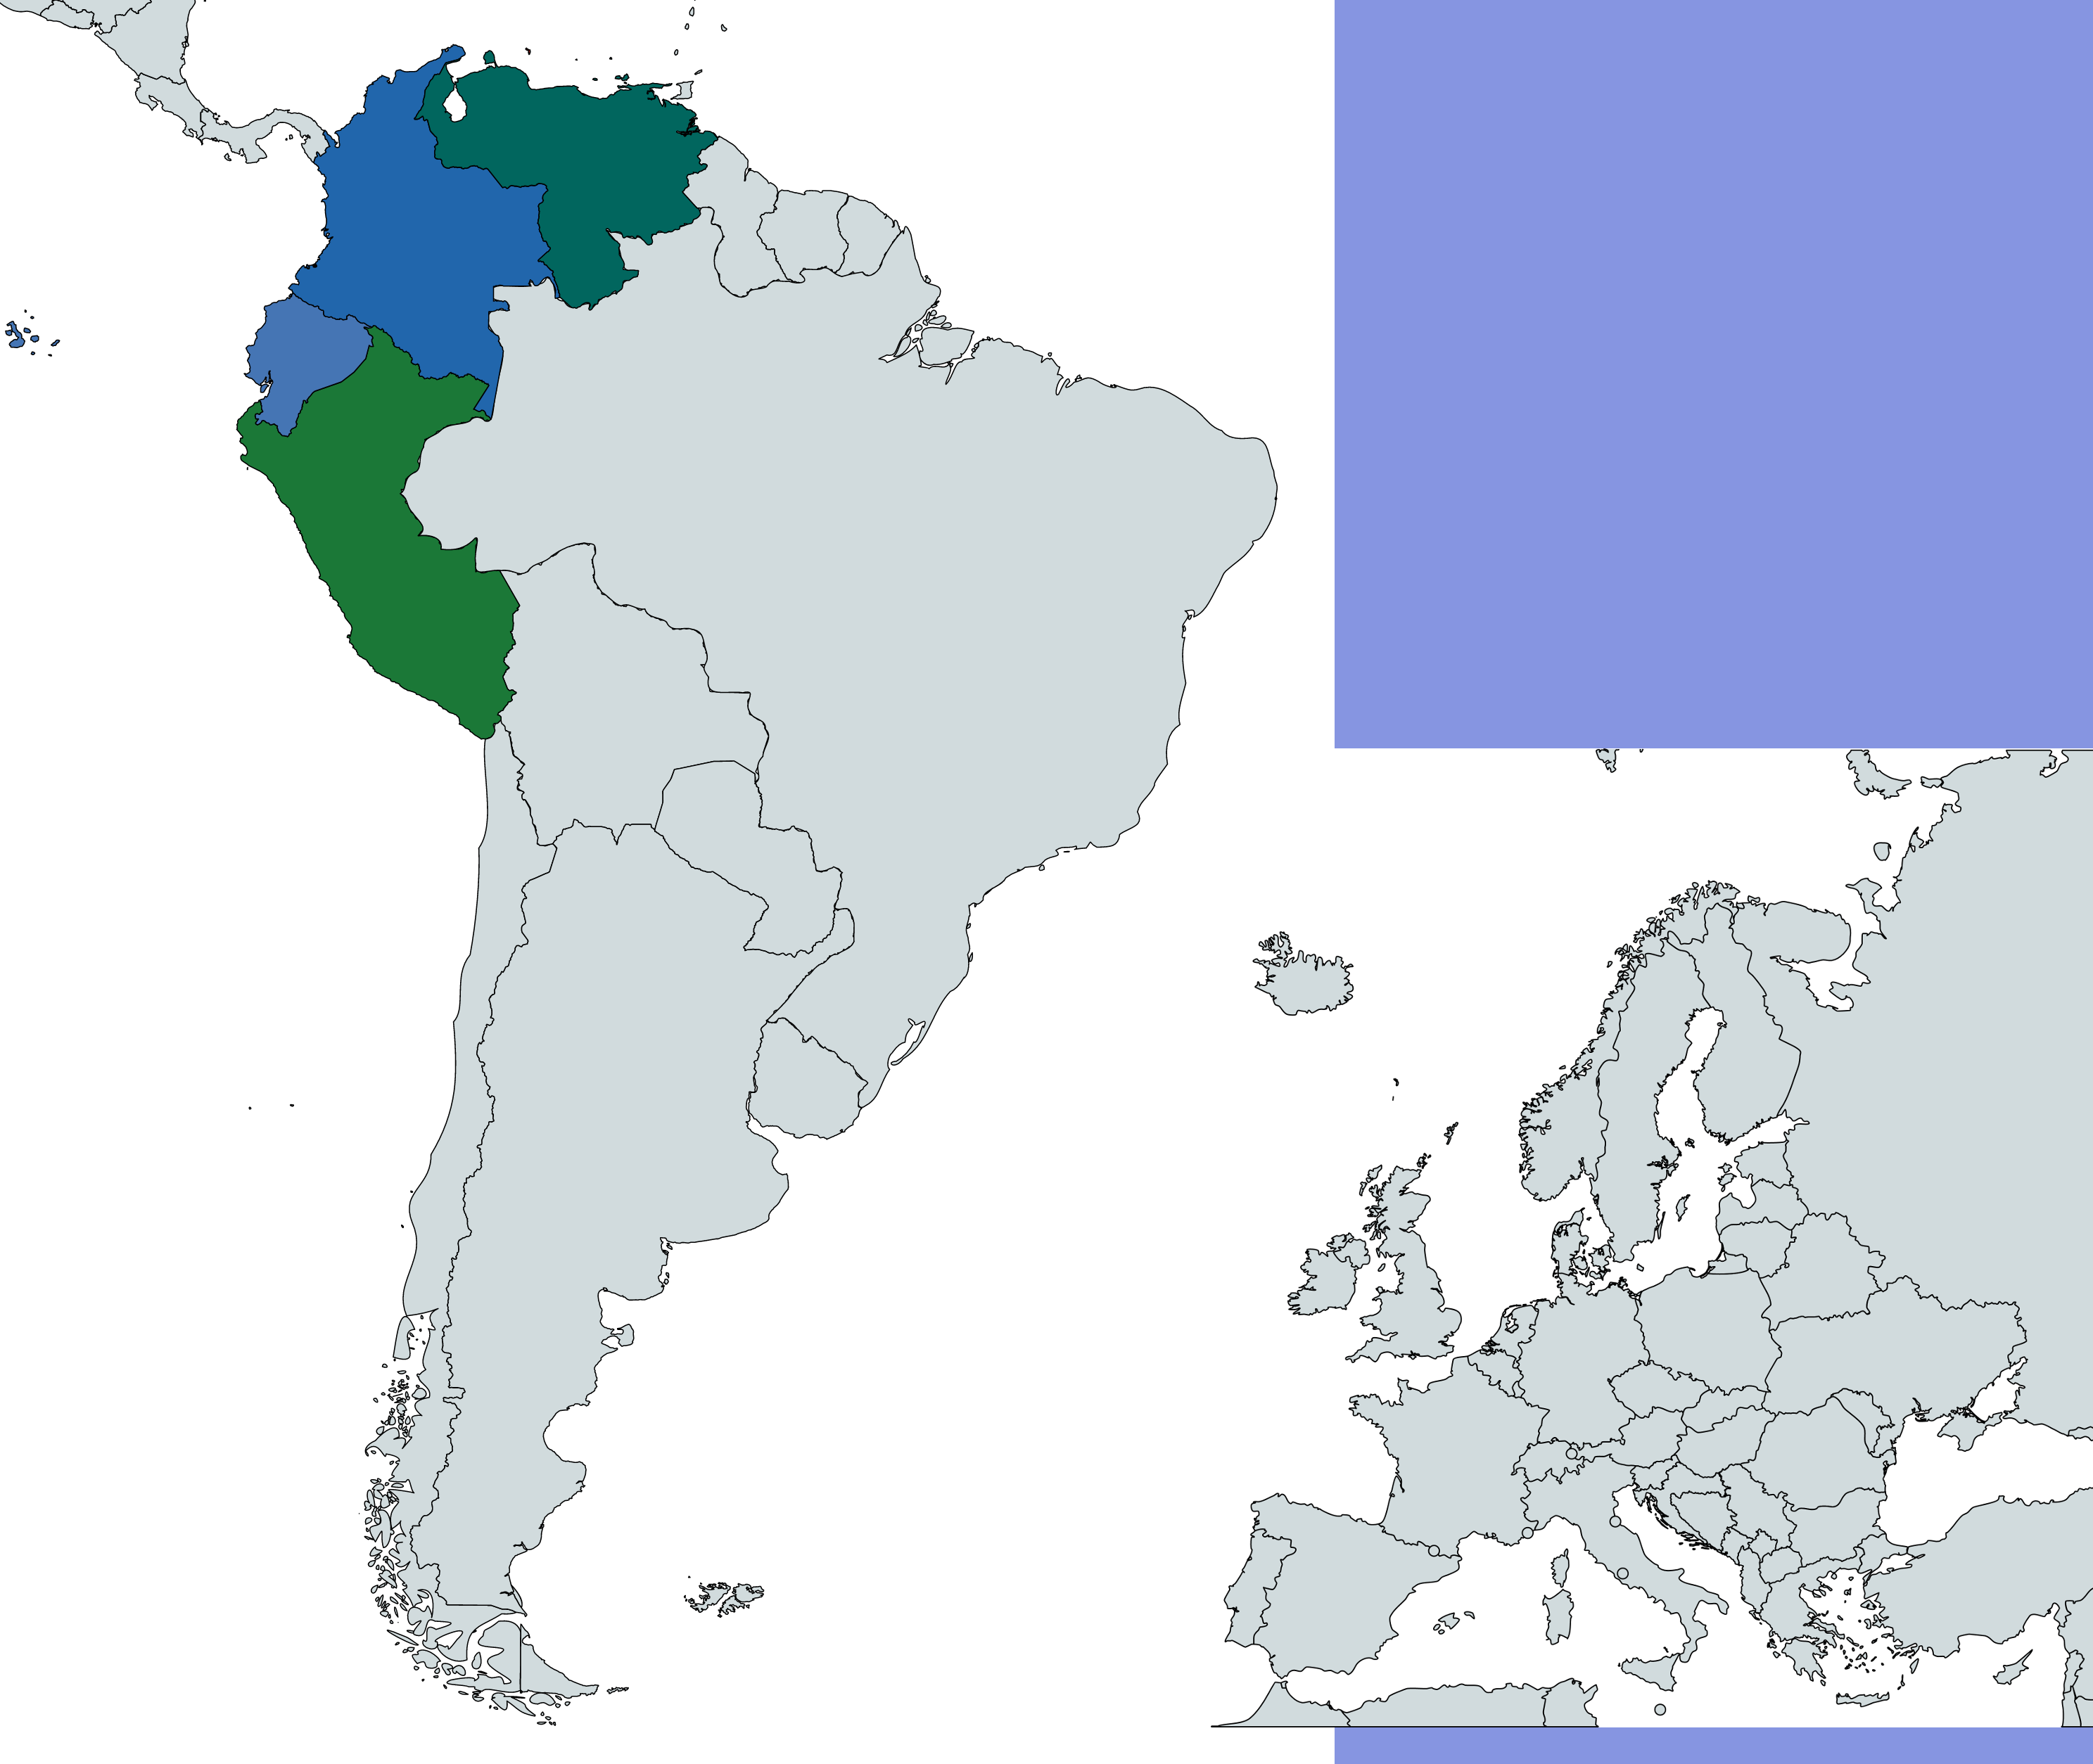
\includegraphics[scale=0.05]{imagenes/mapa_conga_003.png}
\end{center}

\end{columns}



\end{frame}

\begin{frame}[fragile]
\frametitle{Misión, \underline{Visión} y Valores}
\begin{columns}[c] % The "c" option specifies centered vertical alignment while the "t" option is used for top vertical alignment

\column{.58\textwidth}

En LA-CoNGA-physics {\bf \color{LCblueSec1} construimos y cultivamos una red sostenible, dinámica, interconectada y diversa} de investigadores latinoamericanos y europeos en física avanzada, con {\bf \color{LCblueInst} estrechos lazos con el sector productivo, que lidera el desarrollo de la ciencia y la tecnología en la región}. Juntos contribuimos a la modernización, accesibilidad e internacionalización de los sistemas de educación superiores de la región. {\bf\large \color{LCredInst} Nuestra comunidad es una referencia en el contenido curricular, las metodologías educativas utilizadas, e inspira la creación de otras comunidades similares}.

\column{.38\textwidth} % Right column and width
\begin{itemize}
\item Red
\begin{itemize}
\item Sostenible
\item Dinámica
\item Diversa
\end{itemize}
\item Sectores académico y productivo
\item Innovación curricular 
\end{itemize}


\end{columns}



\end{frame}

\begin{frame}[fragile]
\frametitle{Misión, Visión y \underline{Valores}}
\begin{columns}[c] % The "c" option specifies centered vertical alignment while the "t" option is used for top vertical alignment

\column{.32\textwidth}

\begin{itemize}
\item Excelencia
\item Apertura
\item Transparencia
\item Colaboración
\item Respeto
\end{itemize}

\column{.66\textwidth} % Right column and width
Estamos {\bf \color{LCredInst}comprometidos con la \underline{excelencia}, la \underline{apertura} y la \underline{transparencia}} en nuestras actividades educativas y de investigación. {\bf \color{LCblueInst}\underline{Colaboramos}}. Nos comunicamos con palabras, acciones e imágenes que inspiran grandeza, y evitamos las que puedan incomodar a los demás. Fomentamos las discusiones animadas y constructivas. {\bf \color{LCblueSec1}Nos tratamos unos a otros con \underline{respeto} y consideración}.  Acogemos y asesoramos a los miembros nuevos. Fomentamos las ideas novedosas, el debate constructivo. Apoyamos el diálogo entre la teoría y la práctica, entre la academia y la sociedad. {\bf \color{LCblueSec2}\underline{Valoramos} nuestros \underline{orígenes}, \underline{talentos} y \underline{experiencias diversas}}. Siempre estamos abiertos a sugerencias sobre cómo hacerlo mejor.
\end{columns}

\end{frame}